\documentclass[10pt, aspectratio=169]{beamer}

\usepackage{clases}

\title{Investigación Operativa}
\subtitle{Resolución gráfica - Forma estándar - Método de diccionarios}
\date{}
\author{Nazareno Faillace Mullen}
\institute{Departamento de Matemática - FCEN - UBA}
% \titlegraphic{\hfill\includegraphics[height=1.5cm]{logo.pdf}}

\begin{document}

    \maketitle



    \begin{frame}{Resolución gráfica de un problema lineal 2-dimensional}
        Dado un modelo de PL con sólo dos variables, podemos resolverlo gráficamente utilizando algunas herramientas
        básicas. Veamos un ejemplo:
        \[\begin{array}{crl}
              \max & \multicolumn{2}{l}{3x_1+x_2} \\
              \text{s.a:} & x_1+4x_2 \leq   & 8 \\
              & -x_1 + x_2 \leq & 1 \\
              & x_1 \leq        & 5 \\
              & \multicolumn{2}{l}{x_1, x_2 \in \mathbb{R}_{\geq 0}}
        \end{array}
        \]
        Comencemos graficando la región de soluciones factibles
    \end{frame}

    \begin{frame}{}
        \[\{(x_1,x_2)\in\mathbb{R}^2\colon x_1+4x_2 \leq 8\}\]
        \begin{figure}
            \centering
            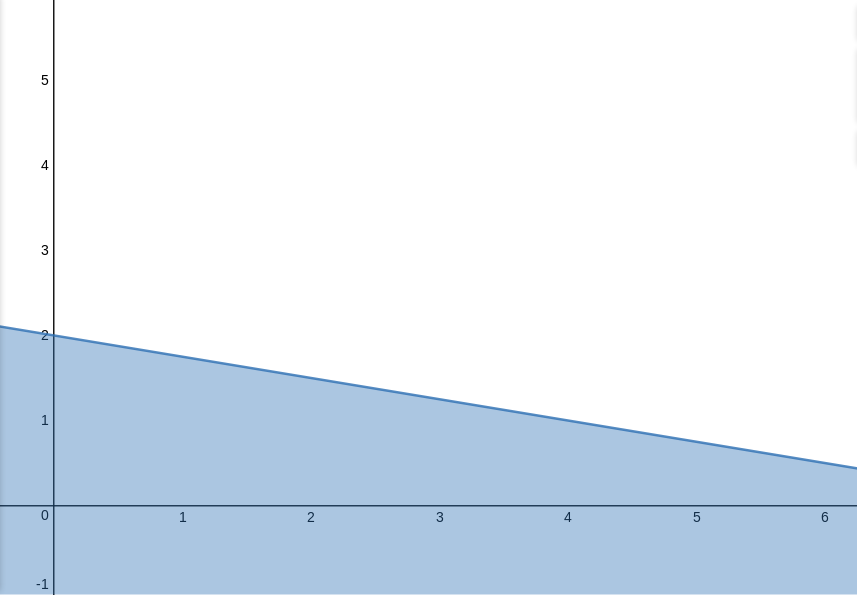
\includegraphics[width=0.78\linewidth]{imagenes/f1.png}
        \end{figure}
    \end{frame}

    \begin{frame}{}
        \[\{(x_1,x_2)\in\mathbb{R}^2\colon x_1+4x_2 \leq 8, -x_1 + x_2 \leq 1 \}\]
        \begin{figure}
            \centering
            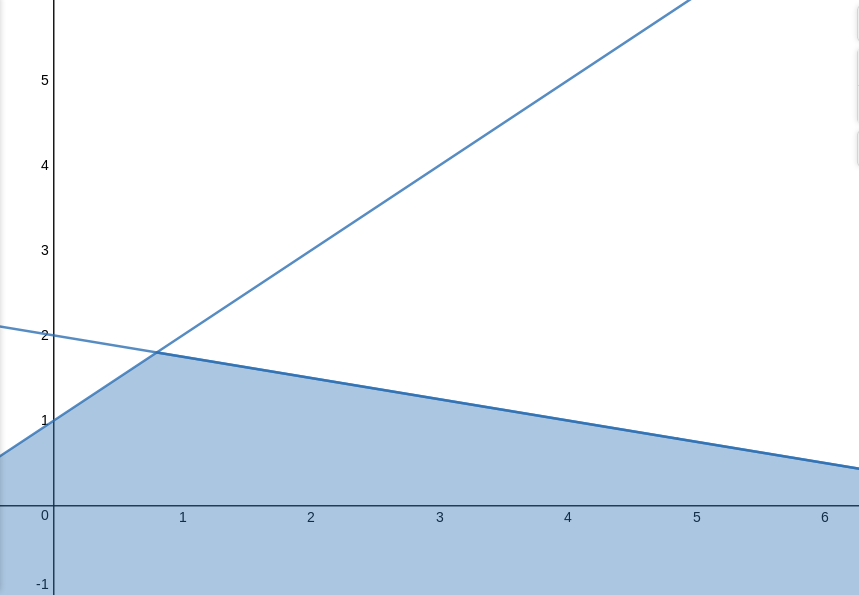
\includegraphics[width=0.78\linewidth]{imagenes/f2.png}
        \end{figure}
    \end{frame}

    \begin{frame}{}
        \[\{(x_1,x_2)\in\mathbb{R}^2\colon x_1+4x_2 \leq 8, -x_1 + x_2 \leq 1, x_1\leq 5 \}\]
        \begin{figure}
            \centering
            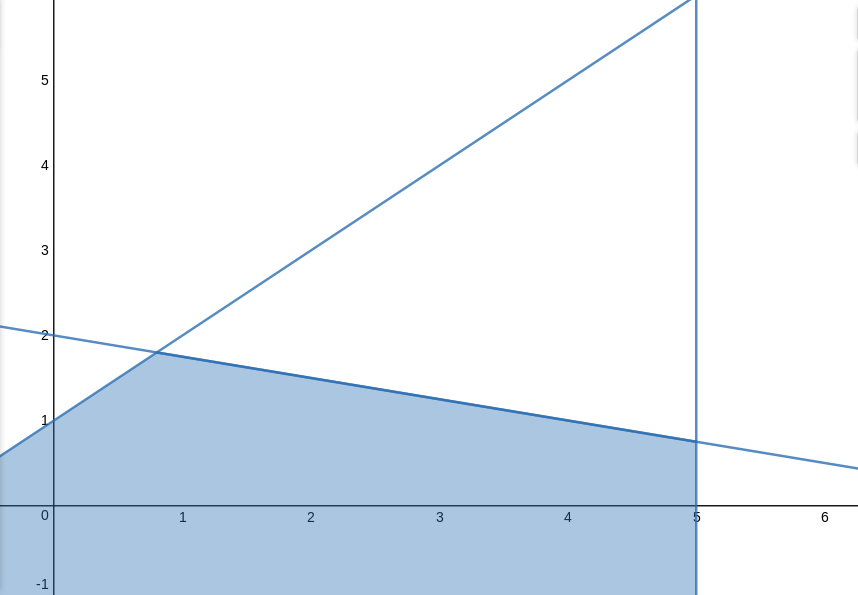
\includegraphics[width=0.8\linewidth]{imagenes/f3.png}
        \end{figure}
    \end{frame}

    \begin{frame}{}
        Región de soluciones factibles:
        \[\{(x_1,x_2)\in\mathbb{R}^2\colon x_1+4x_2 \leq 8, -x_1 + x_2 \leq 1, x_1\leq 5, x_1\geq 0, x_2\geq 0 \}\]
        \begin{figure}
            \centering
            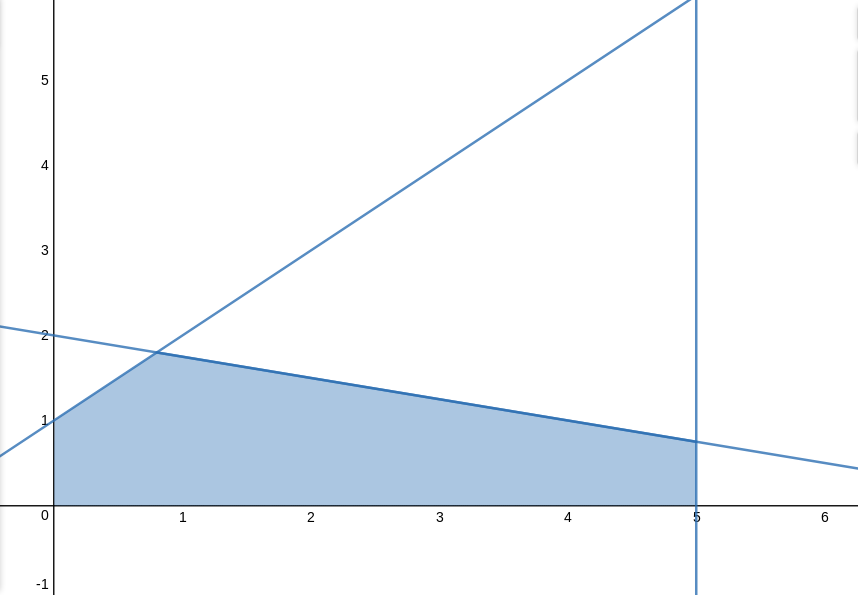
\includegraphics[width=0.8\linewidth]{imagenes/f4.png}
        \end{figure}
    \end{frame}

    \begin{frame}{Resolución gráfica de un problema lineal 2-dimensional}
        Calculamos ahora la dirección de máximo crecimiento, es decir, $\nabla f$, siendo
        $f:\mathbb{R}^2\rightarrow \mathbb{R}$ la f.o.:
        \[ f(x_1,x_2) = 3x_1 + x_2 \Rightarrow \nabla f(x_1,x_2)=(3,1)\]
        Graficamos la curva de nivel $f=0$:
        \[ 0=f(x_1,x_2)=3x_1+x_2 \Leftrightarrow x_2=-3x_1\]
    \end{frame}

    \begin{frame}{}
        \begin{figure}
            \centering
            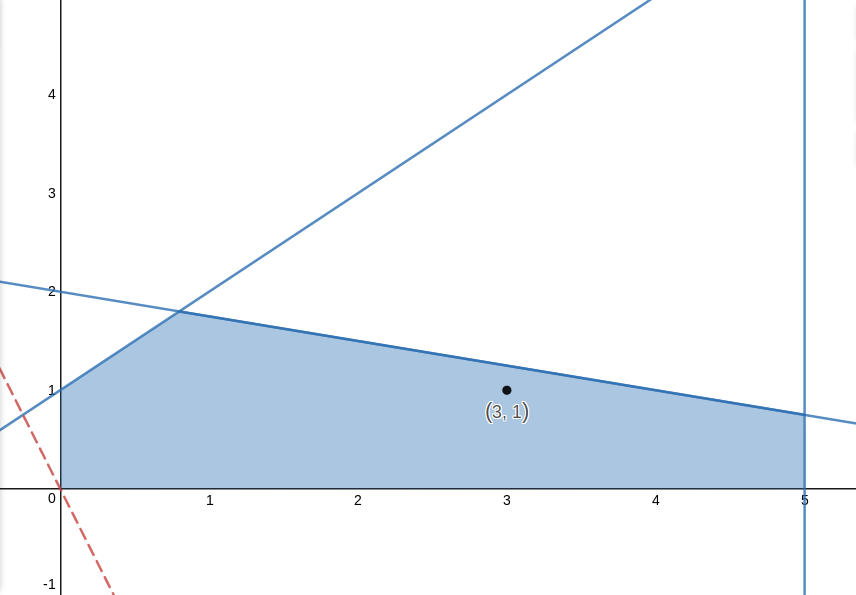
\includegraphics[width=0.8\linewidth]{imagenes/f5.png}
        \end{figure}
    \end{frame}

    \begin{frame}{}
        \begin{figure}
            \centering
            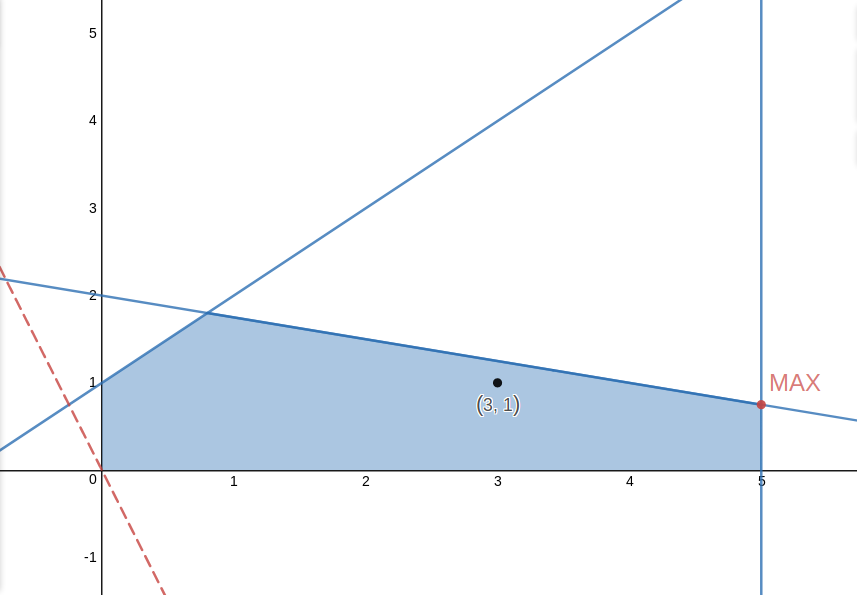
\includegraphics[width=0.8\linewidth]{imagenes/f6.png}
        \end{figure}
    \end{frame}

    \begin{frame}{Resolución gráfica de un problema lineal 2-dimensional}
        Luego, para hallar el máximo basta encontrar la intersección entre $x_1=5$ y $x_1+4x_2=8$:
        \[ \begin{cases}
               x_1=5 \\
               x_1+4x_2=8
        \end{cases} \Rightarrow x_1=5 \; \wedge \; x_2=\dfrac{3}{4}
        \]
        La solución óptima es $(5,\frac{3}{4})$ y el valor óptimo es
        $f(5, \frac{3}{4})= 3\cdot 5 + \frac{3}{4}=\frac{63}{4}$\\
        \vspace{1cm}
        \pause

        El procedimiento para buscar el mínimo es análogo.
    \end{frame}

    \begin{frame}{Resolución gráfica de un problema lineal 2-dimensional}
        \begin{figure}
            \centering
            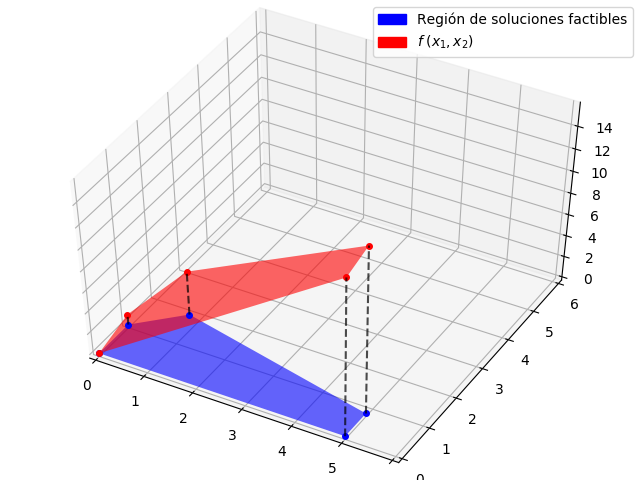
\includegraphics[scale=0.6]{imagenes/Extra.png}
        \end{figure}
    \end{frame}

    \begin{frame}{Resolución gráfica de un problema lineal 2-dimensional}
        Pasos de la resolución gráfica:
        \begin{enumerate}
            \item Graficar la región de soluciones factibles
            \item Calcular $\nabla f$ y la curva de nivel $f=0$
            \item ``Trasladar'' la curva de nivel según corresponda a $\nabla f$
            y al objetivo para % el máximo (mínimo) será el último (primer) vértice que cruce.
            determinar el vértice correspondiente al óptimo.
            \item Hallar los valores de $x_1$ y $x_2$
            correspondientes al óptimo calculando la intersección de las correspondientes restricciones.
        \end{enumerate}


    \end{frame}

    \begin{frame}{Ejemplo}
        Resolver gráficamente:
        \[\begin{array}{crl}
              \min & \multicolumn{2}{l}{2x_1+x_2} \\
              \text{s.a:} & 6x_1-4x_2 \geq & 1 \\
              & x_1 + x_2 \geq & 2 \\
              & x_1 \geq       & 1 \\
              & \multicolumn{2}{l}{x_1, x_2 \in \mathbb{R}_{\geq 0}}
        \end{array}
        \]
    \end{frame}

    \begin{frame}{}
        \begin{figure}
            \centering
            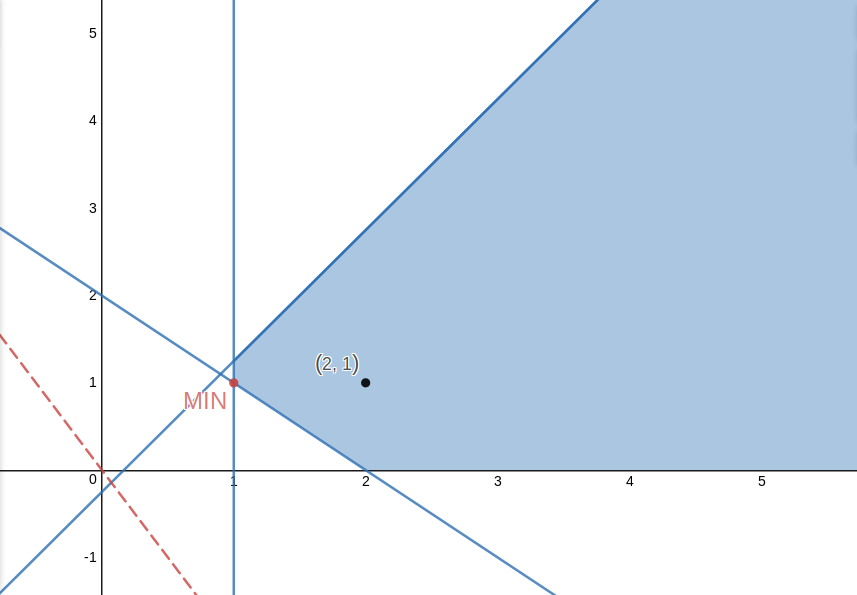
\includegraphics[scale=0.3]{imagenes/f7.png}
        \end{figure}
        \begin{itemize}
            \item La solución óptima es $(1,1)$ y el valor óptimo es $3$.
            \item ¿Y si se hubiese pedido máx en vez de mín? \pause $\rightarrow$ Problema no acotado.
        \end{itemize}
    \end{frame}

    \begin{frame}{Ejemplo - Infinitas soluciones óptimas}
        \[\begin{array}{crl}
              \max & \multicolumn{2}{l}{2x_1+x_2} \\
              \text{s.a:} & x_1 \leq       & 3x_2+1      \\
              & 2x_2 \leq      & -4x_1+18    \\
              & x_1 - x_2 \geq & 0           \\
              & x_1 \geq       & \frac{1}{2} \\
              & \multicolumn{2}{l}{x_1, x_2 \in \mathbb{R}_{\geq 0}}
        \end{array}
        \]
    \end{frame}

    \begin{frame}{}
        \begin{figure}
            \centering
            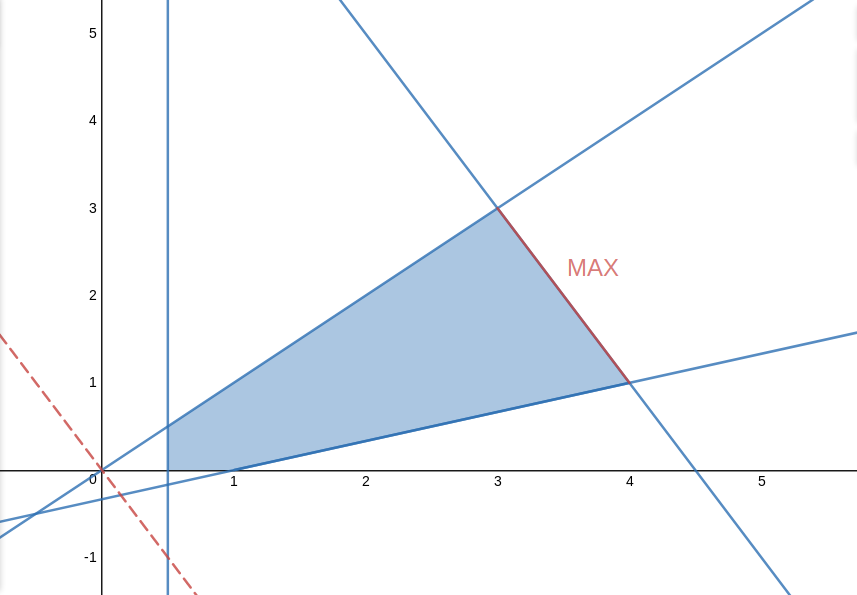
\includegraphics[scale=0.3]{imagenes/f8.png}
        \end{figure}
        \begin{itemize}
            \item Hay infinitas soluciones óptimas: cualquier punto del segmento que une $(3,3)$ con $(4,1)$
            es una solución óptima. El valor óptimo es $9$.
        \end{itemize}
    \end{frame}

    \begin{frame}{Ejemplo - Problema infactible}
        \[\begin{array}{crl}
              \max & \multicolumn{2}{l}{2x_1+5x_2} \\
              \text{s.a:} & x_1 \leq  & 2-x_2 \quad (1)   \\
              & x_2 \geq  & -2x_1+1 \quad (2) \\
              & 4x_1 \geq & 9+x_2 \quad (3)   \\
              & \multicolumn{2}{l}{x_1, x_2 \in \mathbb{R}_{\geq 0}}
        \end{array}
        \]
        \begin{columns}
            \begin{column}{0.5\linewidth}
                \begin{figure}
                    \centering
                    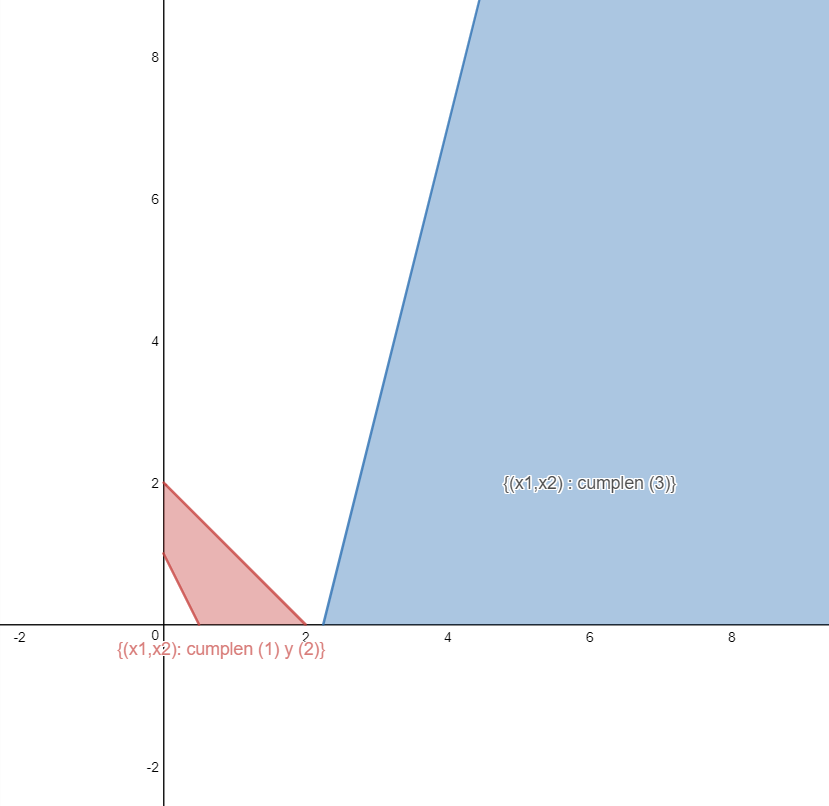
\includegraphics[width=0.8\linewidth]{imagenes/Captura.PNG}
                \end{figure}
            \end{column}
            \begin{column}{0.5\linewidth}
                \begin{itemize}
                    \item No hay soluciones factibles, dado que no existen $(x_1, x_2)$
                    tales que cumplan todas las restricciones.
                \end{itemize}
            \end{column}
        \end{columns}

    \end{frame}

    \begin{frame}{SIMPLEX}
        \large ¿Y si queremos resolver problemas con más de dos variables? \\
        \pause
        Usaremos SIMPLEX, pero harán falta algunas cuentas más
        \centering
        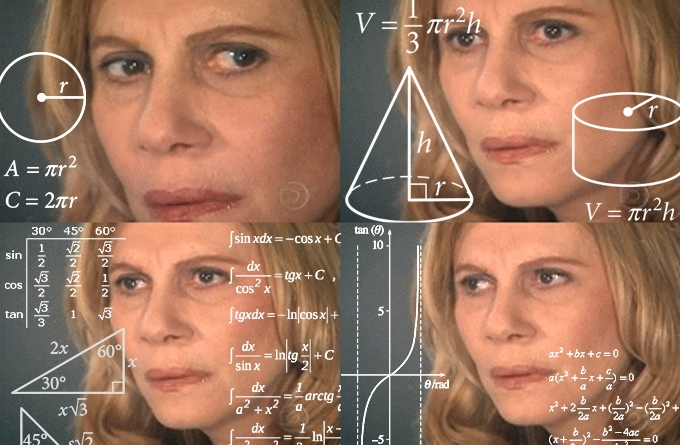
\includegraphics[scale=0.3]{imagenes/bcf.png}
    \end{frame}

    \begin{frame}{Pasar a forma estándar}
        Antes de aplicar cualquiera de los métodos para resolver un modelo de PL con SIMPLEX, debemos pasarlo a forma
        estándar con objetivo de maximizar o minimizar. Debemos asegurarnos que el problema lineal quede planteado de
        alguna de las siguientes maneras:
        \vspace{0.3cm}
        \begin{columns}
            \begin{column}{0.5\linewidth}
                \[
                    \begin{array}{rrl}
                        \min & \multicolumn{2}{l}{c^Tx} \\
                        s.a: & Ax=   & b \\
                        & x\geq & 0
                    \end{array}
                \]
            \end{column}
            \begin{column}{0.5\linewidth}
                \[
                    \begin{array}{rrl}
                        \max & \multicolumn{2}{l}{c^Tx} \\
                        s.a: & Ax=   & b \\
                        & x\geq & 0
                    \end{array}
                \]
            \end{column}
        \end{columns}
        \vspace{0.3cm}
        Con $c, x\in \mathbb{R}^n$, $A\in \mathbb{R}^{m\times n}$ y con $b\in\mathbb{R}^m$ un vector tal que
        $b_i\geq 0 \; \forall i=1,\dots,m$.\\
    \end{frame}

    \begin{frame}{Pasar a forma estándar}
        \begin{itemize}
            \item Si una variable $x_j$ es no positiva, introducimos la variable no negativa $\tilde{x}_j$ al modelo, y
            reemplazamos cada ocurrencia de $x_j$ por $-\tilde{x}_j$
            \item Si una variable $x_j$ es libre (es decir, $x_j\in(-\infty,+\infty)$
            ) agregamos dos variables no negativas $x_j^+$ y $x_j^-$  y reemplazamos cada ocurrencia de $x_j$ por
            $x_j^+ - x_j^-$
            \item Si debemos cambiar el objetivo, basta con cambiarle el signo a la función objetivo:
            \[ \max\; c^Tx \; \leftrightarrow \min\; -c^Tx \]

        \end{itemize}
    \end{frame}

    \begin{frame}{Pasar a forma estándar}
        \begin{itemize}
            \item Si algún $b_i$ es negativo, multiplicamos ambos lados de la igualdad/desigualdad por $-1$:
            \[\begin{array}{rl}
                  \text{si $b_i<0$: } & \displaystyle\sum_j a_{ij}x_j \leq b_i \rightarrow -\sum_j a_{ij}x_j \geq -b_i
                  \\
                  & \displaystyle\sum_j a_{ij}x_j \geq b_i \rightarrow -\sum_j a_{ij}x_j \leq -b_i
            \end{array}\]
            % \[ \text{si $b_i<0$: }\quad \sum_j a_{ij}x_j \leq b_i \rightarrow -\sum_j a_{ij}x_j \geq -b_i \]
            \item Agregamos variables \textit{slack} $w_i$ para transformar las desigualdades en igualdades:
            \[ \sum_j a_{ij}x_j \leq b_i \; \rightarrow \sum_j a_{ij}x_j + w_i = b_i \]
            \[ \sum_j a_{ij}x_j \geq b_i \; \rightarrow \sum_j a_{ij}x_j - w_i = b_i \]
            Se agregan también las restricciones:
            \[w_i\geq 0 \; \forall i\]
        \end{itemize}
    \end{frame}

    \begin{frame}{Ejemplo}
        Pasar a forma estándar (con objetivo de minimizar):
        \[\begin{array}{rrl}
              \max & \multicolumn{2}{l}{x_1 - x_2 + x_3} \\
              \text{s.a:} & x_1 + 2x_2 - x_3 \leq & 3            \\
              & x_1 - x_2 - x_3 \leq  & -2           \\
              & x_1 - x_2 =           & 10           \\
              & x_1\geq               & 0            \\
              & x_2\leq               & 0            \\
              & x_3                   & \text{libre}
        \end{array}
        \]
    \end{frame}


    \begin{frame}{Ejemplo}
        \[\begin{array}{rrl}
              \max & \multicolumn{2}{l}{x_1 - x_2 + x_3} \\
              \text{s.a:} & x_1 + 2x_2 - x_3 \leq & 3            \\
              & x_1 - x_2 - x_3 \leq  & -2           \\
              & x_1 - x_2 =           & 10           \\
              & x_1\geq               & 0            \\
              & \alert{x_2\leq}       & \alert{0}    \\
              & x_3                   & \text{libre}
        \end{array}
        \]
        Como $x_2$ es no positiva, definimos $\tilde{x}_2$ no negativa y reemplazamos $x_2$ por $-\tilde{x}_2$
    \end{frame}

    \begin{frame}{Ejemplo}
        \[\begin{array}{rrl}
              \max & \multicolumn{2}{l}{x_1 \alert{+ \tilde{x}_2} + x_3} \\
              \text{s.a:} & x_1 \alert{-2\tilde{x}_2} - x_3 \leq & 3            \\
              & x_1 \alert{+\tilde{x}_2} - x_3 \leq  & -2           \\
              & x_1 \alert{+\tilde{x}_2} =           & 10           \\
              & x_1\geq                              & 0            \\
              & \alert{\tilde{x}_2 \geq}             & \alert{0}    \\
              & x_3                                  & \text{libre}
        \end{array}
        \]
        Como $x_2$ es no positiva, definimos $\tilde{x}_2$ no negativa y reemplazamos $x_2$ por $-\tilde{x}_2$
    \end{frame}

    \begin{frame}{Ejemplo}
        \[\begin{array}{rrl}
              \max & \multicolumn{2}{l}{x_1 + \tilde{x}_2 + x_3} \\
              \text{s.a:} & x_1 - 2\tilde{x}_2 - x_3 \leq & 3                    \\
              & x_1 + \tilde{x}_2 - x_3 \leq  & -2                   \\
              & x_1 + \tilde{x}_2 =           & 10                   \\
              & x_1\geq                       & 0                    \\
              & \tilde{x}_2 \geq              & 0                    \\
              & \alert{x_3}                   & \alert{\text{libre}}
        \end{array}
        \]
        Como $x_3$ es libre, introducimos las variables no negativas $x_3^+$ y $x_3^-$ y reemplazamos cada ocurrencia de
        $x_3$ por $x_3^+-x_3^-$
    \end{frame}

    \begin{frame}{Ejemplo}
        \[\begin{array}{rrl}
              \max & \multicolumn{2}{l}{x_1 + \tilde{x}_2 + (\alert{x_3^+-x_3^-})} \\
              \text{s.a:} & x_1 - 2\tilde{x}_2 - (\alert{x_3^+-x_3^-}) \leq & 3         \\
              & x_1 + \tilde{x}_2 - (\alert{x_3^+-x_3^-}) \leq  & -2        \\
              & x_1 + \tilde{x}_2 =                             & 10        \\
              & x_1\geq                                         & 0         \\
              & \tilde{x}_2 \geq                                & 0         \\
              & \alert{x_3^+ ,x_3^- \geq}                       & \alert{0}
        \end{array}
        \]
        Como $x_3$ es libre, introducimos las variables no negativas $x_3^+$ y $x_3^-$ y reemplazamos cada ocurrencia de
        $x_3$ por $x_3^+-x_3^-$
    \end{frame}

    \begin{frame}{Ejemplo}
        \[\begin{array}{rrl}
              \max & \multicolumn{2}{l}{x_1 + \tilde{x}_2 + x_3^+-x_3^-} \\
              \text{s.a:} & x_1 - 2\tilde{x}_2 - x_3^++x_3^- \leq & 3  \\
              & x_1 + \tilde{x}_2 - x_3^++x_3^- \leq  & -2 \\
              & x_1 + \tilde{x}_2 =                   & 10 \\
              & x_1\geq                               & 0  \\
              & \tilde{x}_2 \geq                      & 0  \\
              & x_3^+ ,x_3^- \geq                     & 0
        \end{array}
        \]
        Como $x_3$ es libre, introducimos las variables no negativas $x_3^+$ y $x_3^-$ y reemplazamos cada ocurrencia de
        $x_3$ por $x_3^+-x_3^-$
    \end{frame}

    \begin{frame}{Ejemplo}
        \[\begin{array}{rrl}
              \alert{\max} & \multicolumn{2}{l}{\alert{x_1 + \tilde{x}_2 + x_3^+-x_3^-}} \\
              \text{s.a:} & x_1 - 2\tilde{x}_2 - x_3^++x_3^- \leq & 3  \\
              & x_1 + \tilde{x}_2 - x_3^++x_3^- \leq  & -2 \\
              & x_1 + \tilde{x}_2 =                   & 10 \\
              & x_1\geq                               & 0  \\
              & \tilde{x}_2 \geq                      & 0  \\
              & x_3^+ ,x_3^- \geq                     & 0
        \end{array}
        \]
        Como el objetivo es maximizar, lo pasamos a minimizar:
        \[ \max \; x_1 + \tilde{x}_2 + x_3^+-x_3^- \; \rightarrow \min \; -x_1 - \tilde{x}_2 - x_3^++x_3^-\]
    \end{frame}


    \begin{frame}{Ejemplo}
        \[\begin{array}{rrl}
              \mathbf{\min} & \multicolumn{2}{l}{\mathbf{-x_1 - \tilde{x}_2 - x_3^++x_3^-}} \\
              \text{s.a:} & x_1 - 2\tilde{x}_2 - x_3^++x_3^- \leq & 3  \\
              & x_1 + \tilde{x}_2 - x_3^++x_3^- \leq  & -2 \\
              & x_1 + \tilde{x}_2 =                   & 10 \\
              & x_1\geq                               & 0  \\
              & \tilde{x}_2 \geq                      & 0  \\
              & x_3^+ ,x_3^- \geq                     & 0
        \end{array}
        \]
        Como el objetivo es maximizar, lo pasamos a minimizar:
        \[ \max \; x_1 + \tilde{x}_2 + x_3^+-x_3^- \; \rightarrow \min \; -x_1 - \tilde{x}_2 - x_3^++x_3^-\]

%Agregamos la variable slack $w_1$ y pedimos que $w_1\geq 0$:
%\[ x_1 + 2x_2 - x_3 \leq 3 \; \rightarrow x_1 + 2x_2 - x_3 + w_1 = 3 \]
    \end{frame}


    \begin{frame}{Ejemplo}
        \[\begin{array}{rrl}
              \min & \multicolumn{2}{l}{-x_1 - \tilde{x}_2 - x_3^++x_3^-} \\
              \text{s.a:} & \alert{x_1 - 2\tilde{x}_2 - x_3^++x_3^- \leq} & \alert{3} \\
              & x_1 + \tilde{x}_2 - x_3^++x_3^- \leq          & -2        \\
              & x_1 + \tilde{x}_2 =                           & 10        \\
              & x_1\geq                                       & 0         \\
              & \tilde{x}_2 \geq                              & 0         \\
              & x_3^+ ,x_3^- \geq                             & 0
        \end{array}
        \]
        Agregamos la variable slack $w_1$ y pedimos que $w_1\geq 0$:
        \[ x_1 - 2\tilde{x}_2 - x_3^++x_3^- \leq 3 \; \rightarrow x_1 - 2\tilde{x}_2 - x_3^++x_3^- + w_1 = 3 \]
    \end{frame}


    \begin{frame}{Ejemplo}
        \[\begin{array}{rrl}
              \min & \multicolumn{2}{l}{-x_1 - \tilde{x}_2 - x_3^++x_3^-} \\
              \text{s.a:} & \alert{x_1 - 2\tilde{x}_2 - x_3^++x_3^-+w_1 =} & \alert{3} \\
              & x_1 + \tilde{x}_2 - x_3^++x_3^- \leq           & -2        \\
              & x_1 + \tilde{x}_2 =                            & 10        \\
              & x_1\geq                                        & 0         \\
              & \tilde{x}_2 \geq                               & 0         \\
              & x_3^+ ,x_3^- \geq                              & 0         \\
              & \alert{w_1\geq}                                & \alert{0}
        \end{array}
        \]
        Agregamos la variable slack $w_1$ y pedimos que $w_1\geq 0$:
        \[ x_1 - 2\tilde{x}_2 - x_3^++x_3^- \leq 3 \; \rightarrow x_1 - 2\tilde{x}_2 - x_3^++x_3^- + w_1 = 3 \]
    \end{frame}


    \begin{frame}{Ejemplo}
        \[\begin{array}{rrl}
              \min & \multicolumn{2}{l}{-x_1 - \tilde{x}_2 - x_3^++x_3^-} \\
              \text{s.a:} & x_1 - 2\tilde{x}_2 - x_3^++x_3^-+w_1 =       & 3          \\
              & \alert{x_1 + \tilde{x}_2 - x_3^++x_3^- \leq} & \alert{-2} \\
              & x_1 + \tilde{x}_2 =                          & 10         \\
              & x_1\geq                                      & 0          \\
              & \tilde{x}_2 \geq                             & 0          \\
              & x_3^+ ,x_3^- \geq                            & 0          \\
              & w_1\geq                                      & 0
        \end{array}
        \]
        Multiplicamos ambos lados de la desigualdad por $-1$ y luego agregamos la variable slack no negativa:
        \[ x_1 + \tilde{x}_2 - x_3^++x_3^- \leq -2 \quad \rightarrow \quad -x_1 - \tilde{x}_2 + x_3^+-x_3^- \geq 2\]
        \[ -x_1 - \tilde{x}_2 + x_3^+-x_3^- \geq 2 \quad \rightarrow \quad -x_1 - \tilde{x}_2 + x_3^+-x_3^- - w_2 = 2 \]
    \end{frame}


    \begin{frame}{Ejemplo}
        \[\begin{array}{rrl}
              \min & \multicolumn{2}{l}{-x_1 - \tilde{x}_2 - x_3^++x_3^-} \\
              \text{s.a:} & x_1 - 2\tilde{x}_2 - x_3^++x_3^-+w_1 =           & 3         \\
              & \alert{-x_1 - \tilde{x}_2 + x_3^+-x_3^- - w_2 =} & \alert{2} \\
              & x_1 + \tilde{x}_2 =                              & 10        \\
              & x_1\geq                                          & 0         \\
              & \tilde{x}_2 \geq                                 & 0         \\
              & x_3^+ ,x_3^- \geq                                & 0         \\
              & w_1\geq                                          & 0         \\
              & \alert{w_2\geq}                                  & \alert{0} \\

        \end{array}
        \]
        Multiplicamos ambos lados de la desigualdad por $-1$ y luego agregamos la variable slack no negativa:
        \[ x_1 + \tilde{x}_2 - x_3^++x_3^- \leq -2 \rightarrow -x_1 - \tilde{x}_2 + x_3^+-x_3^- \geq 2\]
        \[ -x_1 - \tilde{x}_2 + x_3^+-x_3^- \geq 2 \rightarrow -x_1 - \tilde{x}_2 + x_3^+-x_3^- - w_2 = 2 \]
    \end{frame}

    \begin{frame}{Ejemplo}
        El problema escrito en forma estándar queda entonces:
        \[\begin{array}{rcccccccc}
              \min & \multicolumn{7}{l}{-x_1 - \tilde{x}_2 - x_3^++x_3^-} \\
              \text{s.a:} & x_1  & - 2\tilde{x}_2 & - x_3^+ & +x_3^- & +w_1 &       & =    & 3  \\
              & -x_1 & - \tilde{x}_2  & + x_3^+ & -x_3^- &      & - w_2 & =    & 2  \\
              & x_1  & + \tilde{x}_2  &         &        &      &       & =    & 10 \\
              & x_1, & \tilde{x}_2,   & x_3^+,  & x_3^-, & w_1, & w_2   & \geq & 0
              %  & \multicolumn{7}{l}{x_1\geq 0}\\
              %  & \multicolumn{7}{l}{\tilde{x}_2 \geq 0}\\
              %  & \multicolumn{7}{l}{x_3^+ ,x_3^- \geq 0}\\
              %  & \multicolumn{7}{l}{w_1\geq  0} \\
              %  & \multicolumn{7}{l}{w_2\geq 0}\\
        \end{array}
        \]
        Una vez encontrado el óptimo de este problema mediante SIMPLEX, se puede recuperar la solución óptima para las
        variables del problema original recordando que:
        $$x_2 = -\tilde{x}_2$$
        $$x_3 = x_3^+-x_3^- $$
    \end{frame}

    \begin{frame}{Método de Diccionarios}
        Veremos un ejemplo de cómo utilizar este método con \textbf{objetivo de maximizar}.
        \\
        Problema original:
        \[
            \begin{array}{rrrrrrrr}
                \max & 5x_1 & + & 4x_2 & + & 3x_3 & \\
                \text{s.a:} & 2x_1 & + & 3x_2 & + & x_3  & \leq & 5  \\
                & 4x_1 & + & x_2  & + & 2x_3 & \leq & 11 \\
                & 3x_1 & + & 4x_2 & + & 2x_3 & \leq & 8  \\
                & \multicolumn{5}{r}{x_1,x_2,x_3} & \geq & 0 \\
            \end{array}
        \]
        Problema estandarizado: \pause
        \vspace{0.1cm}
        \[
            \begin{array}{rrrrrrrrrrrrrr}
                \max & 5x_1 & + & 4x_2 & + & 3x_3 & \\
                \text{s.a:} & 2x_1 & + & 3x_2 & + & x_3  & + & w_1 &   &     &   &     & = & 5  \\
                & 4x_1 & + & x_2  & + & 2x_3 &   &     & + & w_2 &   &     & = & 11 \\
                & 3x_1 & + & 4x_2 & + & 2x_3 &   &     &   &     & + & w_3 & = & 8  \\
                & \multicolumn{11}{r}{x_1,x_2,x_3,w_1,w_2,w_3} & \geq & 0 \\
            \end{array}\]
    \end{frame}

    \begin{frame}
        Problema estandarizado:
        \vspace{0.1cm}
        \[
            \begin{array}{rrrrrrrrrrrrrr}
                \max & 5x_1 & + & 4x_2 & + & 3x_3 & \\
                \text{s.a:} & 2x_1 & + & 3x_2 & + & x_3  & + & w_1 &   &     &   &     & = & 5  \\
                & 4x_1 & + & x_2  & + & 2x_3 &   &     & + & w_2 &   &     & = & 11 \\
                & 3x_1 & + & 4x_2 & + & 2x_3 &   &     &   &     & + & w_3 & = & 8  \\
                & \multicolumn{11}{r}{x_1,x_2,x_3,w_1,w_2,w_3} & \geq & 0 \\
        \end{array}\]

        \[
            A = \begin{pmatrix}
                    2 & 3 & 1 & 1 & 0 & 0 \\
                    4 & 1 & 2 & 0 & 1 & 0 \\
                    3 & 4 & 2 & 0 & 0 & 1 \\
            \end{pmatrix}
        \]

        \textbf{Obs:} $rango(A)=3$
    \end{frame}

    \begin{frame}
        \[
            \begin{pmatrix}
                    2 & 3 & 1 & 1 & 0 & 0 \\
                    4 & 1 & 2 & 0 & 1 & 0 \\
                    3 & 4 & 2 & 0 & 0 & 1 \\
            \end{pmatrix}
            \begin{pmatrix}
                x_1 \\
                x_2 \\
                x_3 \\
                w_1 \\
                w_2 \\
                w_3
            \end{pmatrix} =
            \begin{pmatrix}
                5 \\
                11 \\
                8
            \end{pmatrix} \iff
        \]

        \[\iff
        \begin{pmatrix}
            2 \\
            4 \\
            3 \\
        \end{pmatrix} x_1 +
        \begin{pmatrix}
            3 \\
            1 \\
            4 \\
        \end{pmatrix} x_2 +
        \begin{pmatrix}
            1 \\
            2 \\
            2 \\
        \end{pmatrix} x_3 +
        \begin{pmatrix}
            1 \\
            0 \\
            0 \\
        \end{pmatrix} w_1 +
        \begin{pmatrix}
            0 \\
            1 \\
            0 \\
        \end{pmatrix} w_2 +
        \begin{pmatrix}
            0 \\
            0 \\
            1 \\
        \end{pmatrix} w_3 =
        \begin{pmatrix}
                5 \\
                11 \\
                8
        \end{pmatrix}
        \]

        $\Rightarrow$ $b$ es combinación lineal de las columnas de $A$.
        \vspace{1em}

        \textbf{Obs:} si tomo 3 columnas de $A$ que sean l.i., tengo una \textbf{base} de $\mathbb{R}^3$

    \end{frame}

    \begin{frame}
        \textbf{Ejemplo:} las columnas
        \[
        \begin{pmatrix}
            1 \\
            2 \\
            2 \\
        \end{pmatrix}
        \begin{pmatrix}
            1 \\
            0 \\
            0 \\
        \end{pmatrix}
        \begin{pmatrix}
            0 \\
            1 \\
            0 \\
        \end{pmatrix}
        \]
        son base de $\mathbb{R}^3$, entonces podemos escribir $b$ como combinación lineal de ellas:
        \pause
        \[
        \begin{pmatrix}
            1 \\
            2 \\
            2 \\
        \end{pmatrix} \underbrace{4}_{x_3} +
        \begin{pmatrix}
            1 \\
            0 \\
            0 \\
        \end{pmatrix} \underbrace{1}_{w_1} +
        \begin{pmatrix}
            0 \\
            1 \\
            0 \\
        \end{pmatrix} \underbrace{3}_{w_2} =
        \begin{pmatrix}
                5 \\
                11 \\
                8
        \end{pmatrix}
        \]
        Esto significa que $x_3=4,w_1=1,w_2=3$ y el resto de las variables es $0$. Como en este caso todas las
        variables valen $\geq 0$, el vector:
        \[(x_1,x_2,x_3,w_1,w_2,w_3)=(0,0,4,1,3,0)\]
        es una \textbf{solución básica factible}. \pause

        Decimos que $x_3,w_1,w_2$ son las \textbf{variables básicas} de esa solución, pues corresponden a las
        columnas de $A$ que elegimos para formar una base de $\mathbb{R}^3$. Mientras
        que $x_1,x_2,w_3$ son
        \textbf{variables no básicas}.
    \end{frame}

    \begin{frame}
        \textbf{Ejemplo:} las columnas
        \[
        \begin{pmatrix}
            3 \\
            1 \\
            4 \\
        \end{pmatrix}
        \begin{pmatrix}
            1 \\
            2 \\
            2 \\
        \end{pmatrix}
        \begin{pmatrix}
            0 \\
            0 \\
            1 \\
        \end{pmatrix}
        \]
        son base de $\mathbb{R}^3$, entonces podemos escribir $b$ como combinación lineal de ellas:
        \pause
        \[
        \begin{pmatrix}
            3 \\
            1 \\
            4 \\
        \end{pmatrix} \underbrace{\left(-\dfrac{1}{5}\right)}_{x_2} +
        \begin{pmatrix}
            1 \\
            2 \\
            2 \\
        \end{pmatrix} \underbrace{\dfrac{28}{5}}_{x_3} +
        \begin{pmatrix}
            0 \\
            0 \\
            1 \\
        \end{pmatrix} \underbrace{\left(-\dfrac{12}{5}\right)}_{w_3} =
        \begin{pmatrix}
                5 \\
                11 \\
                8
        \end{pmatrix}
        \]
        Esto significa que $x_2=-\dfrac{1}{5},x_3=\dfrac{28}{5},w_2=-\dfrac{12}{5}$ y el resto de las variables es $0$.

        ¿Podemos decir que $(0,-\frac{1}{5},\frac{28}{5},0,0,-\frac{12}{5})$ es una solución básica factible?
    \end{frame}

    \begin{frame}
        En general, si $A\in\mathbb{R}^{m\times n}$ con $n>m$ y tal que $rango(A)=m$, en el peor de los casos tenemos
        $\binom{n}{m}$ posibles bases.

        En nuestro ejemplo, podrían haber hasta \textbf{20 bases}.
        \pause

        SIMPLEX es un algoritmo que (generalmente) evita tener que enumerarlas a todas.
    \end{frame}

    \begin{frame}{Método de Diccionarios}
        Problema estandarizado:
        \vspace{0.3cm}
        \[
            \begin{array}{rrrrrrrrrrrrrr}
                \max & 5x_1 & + & 4x_2 & + & 3x_3 & \\
                \text{s.a:} & 2x_1 & + & 3x_2 & + & x_3  & + & w_1 &   &     &   &     & = & 5  \\
                & 4x_1 & + & x_2  & + & 2x_3 &   &     & + & w_2 &   &     & = & 11 \\
                & 3x_1 & + & 4x_2 & + & 2x_3 &   &     &   &     & + & w_3 & = & 8  \\
                & \multicolumn{11}{r}{x_1,x_2,x_3,w_1,w_2,w_3} & \geq & 0 \\
            \end{array}\]
%    \vspace{0.2cm}

        Una vez estandarizado, notamos con $z$ a la f.o. y pasamos las variables no básicas
        (en este caso, las $x$) al lado derecho de la igualdad.
        % Cada elección de $x_1, x_2, x_3$ define los valores de $w_1,w_2,w_3$ y $z$.
        % \begin{array}{rrrrrrrrr}
        %      & = & & & & & & & \\
        %      & = & & & & & & & \\
        %      & = & & & & & & & \\
        %     z & = & & & & & & & \\
        % \end{array}

        \[
            \begin{array}{rrrrrrrrr}

                w_1 & = & 5  & - & 2x_1 & - & 3x_2 & - & x_3  \\
                w_2 & = & 11 & - & 4x_1 & - & x_2  & - & 2x_3 \\
                w_3 & = & 8  & - & 3x_1 & - & 4x_2 & - & 2x_3 \\\hline
                z   & = &    &   & 5x_1 & + & 4x_2 & + & 3x_3 \\
            \end{array}
        \]
    \end{frame}

    \begin{frame}{Método de Diccionarios}
        Problema estandarizado:
        \vspace{0.3cm}
        \[
            \begin{array}{rrrrrrrrrrrrrr}
                \max & 5x_1 & + & 4x_2 & + & 3x_3 & \\
                \text{s.a:} & 2x_1 & + & 3x_2 & + & x_3  & + & w_1 &   &     &   &     & = & 5  \\
                & 4x_1 & + & x_2  & + & 2x_3 &   &     & + & w_2 &   &     & = & 11 \\
                & 3x_1 & + & 4x_2 & + & 2x_3 &   &     &   &     & + & w_3 & = & 8  \\
                & \multicolumn{11}{r}{x_1,x_2,x_3,w_1,w_2,w_3} & \geq & 0 \\
            \end{array}\]
%     \vspace{0.3cm}
        Una vez estandarizado, notamos con $z$ a la f.o. y pasamos las variables no básicas (en este caso, las $x$)
        %de decisión
        al lado derecho de la igualdad. % Cada elección de $x_1, x_2, x_3$ define los valores de $w_1,w_2,w_3$ y $z$.
        % \begin{array}{rrrrrrrrr}
        %      & = & & & & & & & \\
        %      & = & & & & & & & \\
        %      & = & & & & & & & \\
        %     z & = & & & & & & & \\
        % \end{array}
        \[
            \begin{array}{rrrrrrrll}

                \text{\textcolor{blue}{$\pmb{w_1}$}} & = & 5  & - & 2\text{\textcolor{red}{$\pmb{x_1}$}} & - & 3
                \text{\textcolor{red}{$\pmb{x_2}$}} & - & \text{\textcolor{red}{$\pmb{x_3}$}} \\
                \text{\textcolor{blue}{$\pmb{w_2}$}} & = & 11 & - & 4\text{\textcolor{red}{$\pmb{x_1}$}} & - &
                \text{\textcolor{red}{$\pmb{x_2}$}} & - & 2\text{\textcolor{red}{$\pmb{x_3}$}} \\
                \text{\textcolor{blue}{$\pmb{w_3}$}} & = & 8  & - & 3\text{\textcolor{red}{$\pmb{x_1}$}} & - & 4
                \text{\textcolor{red}{$\pmb{x_2}$}} & - & 2\text{\textcolor{red}{$\pmb{x_3}$}} \\\hline
                z                                    & = &    &   & {\color{goodgreen}\pmb{5}}x_1        & + &
                    {\color{goodgreen}\pmb{4}}x_2        & + & {\color{goodgreen}\pmb{3}}x_3        \\
                \text{\textcolor{blue}{Variables básicas}} & &
                \multicolumn{5}{l}{\text{\textcolor{red}{Variables no básicas}}} &
                \multicolumn{2}{l}{\text{\textcolor{goodgreen}{Costos reducidos}}}
            \end{array}
        \]

    \end{frame}

    \begin{frame}{}
        \[
            \begin{array}{rrrrrrrrr}
                w_1 & = & 5  & - & 2x_1 & - & 3x_2 & - & x_3  \\
                w_2 & = & 11 & - & 4x_1 & - & x_2  & - & 2x_3 \\
                w_3 & = & 8  & - & 3x_1 & - & 4x_2 & - & 2x_3 \\\hline
                z   & = &    &   & 5x_1 & + & 4x_2 & + & 3x_3 \\
            \end{array}
        \]
%        Para comenzar a resolver el problema lineal, necesitamos una solución básica factible
%        $x_1,x_2,x_3, w_1, w_2.w_3$. En nuestro ejemplo, podemos comenzar tomando $x_1=x_2=x_3=0$ (pues cumple que
%        $w_i\geq 0$). Luego, nuestra solución inicial es:
        Nuestra solución básica factible inicial es:
        \[x_1=0,\; x_2=0,\; x_3=0,\; w_1=5,\; w_2=11,\; w_3=8\;\]
        lo cual da como resultado $z=0$. Nos gustaría hallar otra solución factible que aumente el valor de $z$.\\
        \pause
        Como $x_1$ tiene el \textbf{mayor coeficiente en $z$}, parece una buena idea intentar
        \textbf{aumentar el valor de $x_1$}.

    \end{frame}

    \begin{frame}{}
        \small
        \[
            \begin{array}{rrrrrrrrr}
                w_1 & = & 5  & - & 2x_1 & - & 3x_2 & - & x_3  \\
                w_2 & = & 11 & - & 4x_1 & - & x_2  & - & 2x_3 \\
                w_3 & = & 8  & - & 3x_1 & - & 4x_2 & - & 2x_3 \\\hline
                z   & = &    &   & 5x_1 & + & 4x_2 & + & 3x_3 \\
            \end{array}
        \]
        \textbf{Fijamos $\mathbf{x_2=x_3=0}$} y aumentamos $x_1$. Cada ecuación $i$ nos acota el valor que puede tomar
        $x_1$ de manera tal que $w_i\geq0$:
        \[ 0\leq w_1 = 5-2x_1 \Rightarrow x_1 \leq \frac{5}{2} \]
        \[ 0\leq w_2 = 11-4x_1 \Rightarrow x_1 \leq \frac{11}{4} \]
        \[ 0\leq w_3 = 8-3x_1 \Rightarrow x_1 \leq \frac{8}{3} \]
        \pause
        \textbf{La cota relevante es la más restrictiva}. En este caso, es la primera. Entonces, aumentamos $x_1$ hasta
        $\frac{5}{2}$. Esto hace que $w_1$ disminuya hasta $0$.
    \end{frame}

    \begin{frame}{}
        \small
%        Queremos seguir buscando mejores soluciones. Para eso, tenemos que
%        \textbf{escribir a las variables que sean positivas en función de las variables que valen 0}
%        , como habíamos hecho al principio.\\

        Como $x_1$ dejó de valer $0$, debe pasar al lado izquierdo (\textbf{entra a la base}),
        mientras que $w_1$, que ahora vale $0$, debe pasar al lado derecho (\textbf{sale de la base}).
        De la primera ecuación del diccionario obtenemos que:
        \[ w_1  =  5 - 2x_1 - 3x_2 - x_3 \quad \Rightarrow \quad x_1 = \frac{5}{2} - \frac{3}{2}x_2 -\frac{1}{2}x_3 -
        \frac{1}{2} w_1  \]
        Luego, reemplazamos $x_1$ por la igualdad de arriba en las ecuaciones 2 y 3 y en $z$:
        \[ w_2 = 11 - 4\left(\frac{5}{2} - \frac{3}{2}x_2 -\frac{1}{2}x_3 -\frac{1}{2} w_1 \right)
        - x_2 - 2x_3 = 1+5x_2+2w_1  \]
        \[w_3 = 8 - 3\left(\frac{5}{2} - \frac{3}{2}x_2 -\frac{1}{2}x_3 -\frac{1}{2} w_1 \right) - 4x_2 - 2x_3 =
        \frac{1}{2}+\frac{1}{2}x_2-\frac{1}{2}x_3+\frac{3}{2}w_1\]
        \[z  = 5\left(\frac{5}{2} - \frac{3}{2}x_2 -\frac{1}{2}x_3 -\frac{1}{2} w_1\right) + 4x_2 + 3x_3 = \frac{25}{2}-
        \frac{7}{2}x_2+\frac{1}{2}x_3-\frac{5}{2}w_1 \]

        % \[
        % \begin{array}{rrrrrrrrr}
        %     x_1 & =& \frac{5}{2} &-& \frac{3}{2}x_2& -&\frac{1}{2}x_3& -&\frac{1}{2} w_1 \\
        %     w_2 & = & 11 & - & 4\left(\frac{5}{2} - \frac{3}{2}x_2 -\frac{1}{2}x_3 -\frac{1}{2} w_1 \right) & - &
        %     x_2 & - & 2x_3 \\
        %     w_3 & = & 8 & - & 3\left(\frac{5}{2} - \frac{3}{2}x_2 -\frac{1}{2}x_3 -\frac{1}{2} w_1 \right) & - &
        %     4x_2 & - & 2x_3 \\
        %     z & = & & & 5\left(\frac{5}{2} - \frac{3}{2}x_2 -\frac{1}{2}x_3 -\frac{1}{2} w_1\right)& + & 4x_2 & + &
        %     3x_3 \\
        % \end{array}
        % \]
    \end{frame}

    \begin{frame}{}
        Nuestro nuevo diccionario queda:
        \[
            \begin{array}{rrrrrrrrr}
                x_1 & = & \frac{5}{2}  & - & \frac{3}{2}x_2 & - & \frac{1}{2}x_3 & - & \frac{1}{2} w_1 \\
                w_2 & = & 1            & + & 5x_2           &   &                & + & 2w_1            \\
                w_3 & = & \frac{1}{2}  & + & \frac{1}{2}x_2 & - & \frac{1}{2}x_3 & + & \frac{3}{2}w_1  \\\hline
                z   & = & \frac{25}{2} & - & \frac{7}{2}x_2 & + & \frac{1}{2}x_3 & - & \frac{5}{2}w_1  \\
            \end{array}
        \]
        En el diccionario podemos ver que la solución actual es:
        \[x_1=\frac{5}{2},\; x_2=0,\; x_3=0,\; w_1=0,\; w_2=1,\; w_3=\frac{1}{2}\;\]
        Con valor en la función objetivo:
        \[z=\frac{25}{2}\]\pause
        Si queremos aumentar el valor de $z$, nuestra única opción es incrementar el valor de $x_3$ fijando $x_2=w_1=0$.
        Luego, $x_3$ entrará a la base.
    \end{frame}

    \begin{frame}
        De nuevo, tenemos que ver cuánto podemos aumentarlo para que se respete $x_1, w_2, w_3 \geq 0$:

        \[ 0\leq x_1 = \frac{5}{2}-\frac{1}{2}x_3 \Rightarrow x_3 \leq 5 \]
        \[ 0\leq w_2 = 1+0x_3 \Rightarrow x_3 < \infty \]
        \[ 0\leq w_3 = \frac{1}{2}-\frac{1}{2}x_3 \Rightarrow \mathbf{x_3 \leq 1} \]

        Como la tercera es la condición más restrictiva, $x_3$ entra a la base y $w_3$ sale de la base.
    \end{frame}

    \begin{frame}{}
        \small
        De la tercera ecuación, teníamos que:
        \[w_3 = \frac{1}{2}+\frac{1}{2}x_2-\frac{1}{2}x_3+\frac{3}{2}w_1 \Rightarrow x_3=1+x_2+3w_1-2w_3\]
        Reemplazando $x_3$ por esa expresión en las demás ecuaciones, nos queda el siguiente diccionario:
        \[
            \begin{array}{rrrrrrrrr}
                x_3 & = & 1  & + & x_2  & + & 3w_1 & - & 2w_3 \\
                x_1 & = & 2  & - & 2x_2 & - & 2w_1 & + & w_3  \\
                w_2 & = & 1  & + & 5x_2 & + & 2w_1 &   &      \\\hline
                z   & = & 13 & - & 3x_2 & - & w_1  & - & w_3  \\
            \end{array}
        \]
        Nuestra nueva solución es:
        \[x_1=2,\; x_2=0,\; x_3=1,\; w_1=0,\; w_2=1,\; w_3=0\;\]
        y su valor en la f.o. es $13$.\\
        % Ahora elegimos qué variable del lado derecho aumentar para que incremente el valor de $z$. \pause Pero...
        % ¡cualquier incremento que hagamos sobre esas variables implica la disminución de $z$!
    \end{frame}

    \begin{frame}{}
        \small
        \[\begin{array}{rrrrrrrrr}
              x_3 & = & 1  & + & x_2  & + & 3w_1 & - & 2w_3 \\
              x_1 & = & 2  & - & 2x_2 & - & 2w_1 & + & w_3  \\
              w_2 & = & 1  & + & 5x_2 & + & 2w_1 &   &      \\\hline
              z   & = & 13 & - & 3x_2 & - & w_1  & - & w_3  \\
        \end{array}
        \]
        Ahora elegimos qué variable del lado derecho aumentar para que incremente el valor de $z$. \pause
        Pero... ¡cualquier incremento que hagamos sobre esas variables implica la disminución de $z$! $\Rightarrow$
        ¡Llegamos a un óptimo! \\
        Una solución óptima al problema estandarizado es:
        \[x_1=2,\; x_2=0,\; x_3=1,\; w_1=0,\; w_2=1,\; w_3=0\;\]
        Luego, una solución óptima al problema original es:
        \[x_1=2,\; x_2=0,\; x_3=1\]
        ¿Cómo sabemos que llegamos a un óptimo?\\
        Estamos maximizando y no hay costos reducidos positivos.
%        Tendríamos que ver que $z\leq 13$. Bueno, en la última línea teníamos que:
%        \[z = 13 - 3x_2 - w_1 - w_3\]
%        Como $x_2,w_1,w_3\geq 0$, se tiene necesariamente que $z\leq13$. Como encontramos una solución factible tal que
%        $z=13$, esa solución es óptima.
    \end{frame}

    \begin{frame}{Método de Diccionarios}

        Recapitulando, el procedimiento para aplicar SIMPLEX con el método de diccionarios para un problema con objetivo
        maximizar (\alert{minimizar}):
        \begin{enumerate}
            \item Estandarizar el problema lineal %(con objetivo de \textbf{maximizar})
            \item Hallar solución factible inicial (*)
            \item Escribir el diccionario dejando del lado izquierdo a las variables básicas. %no nulas de la solución
            \item Mientras hayan coeficientes de la f.o. ($z$) positivos (\alert{negativos}):
            \begin{enumerate}

                \item Elegir qué variable no básica aumentar, es decir, qué variable entra a la base (siempre alguna con
                coeficiente positivo (\alert{negativo}) en $z$)
                \item Calcular cuánto puede aumentar dicha variable y cuál es la variable que sale de la base
                (\textit{Pivote})
                \item Escribir el nuevo diccionario con las variables básicas en función de las no básicas.
                (\textit{Pivotear})
            \end{enumerate}
        \end{enumerate}
    \end{frame}

    \begin{frame}{Método de Diccionarios}
        Observemos nuestro recorrido de soluciones a lo largo de la aplicación de SIMPLEX:
        \[ x_1=0, \quad x_2=0, \quad x_3=0 \]
        \begin{figure}
            \centering
            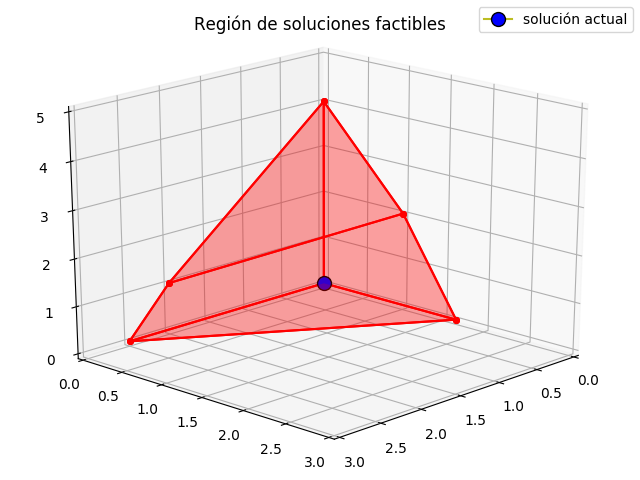
\includegraphics[scale=0.5]{imagenes/s1.png}
        \end{figure}
    \end{frame}

    \begin{frame}{Método de Diccionarios}
        Observemos nuestro recorrido de soluciones a lo largo de la aplicación de SIMPLEX:
        \[ x_1=\frac{5}{2}, \quad x_2=0, \quad x_3=0 \]
        \begin{figure}
            \centering
            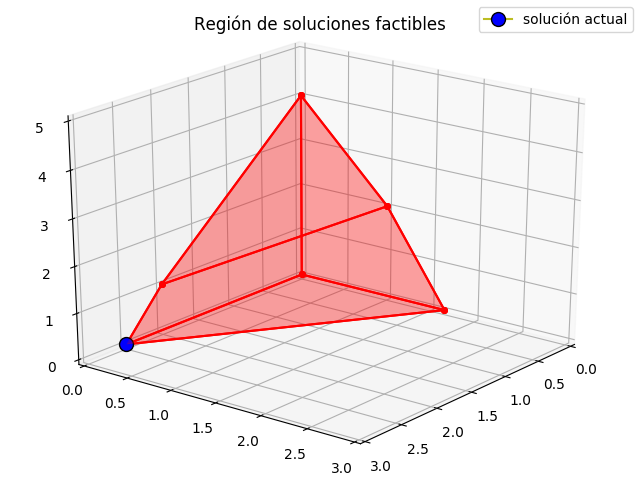
\includegraphics[scale=0.5]{imagenes/s2.png}
        \end{figure}
    \end{frame}

    \begin{frame}{Método de Diccionarios}
        Observemos nuestro recorrido de soluciones a lo largo de la aplicación de SIMPLEX:
        \[ x_1=2, \quad x_2=0, \quad x_3=1 \quad \text{(solución óptima)} \]
        \begin{figure}
            \centering
            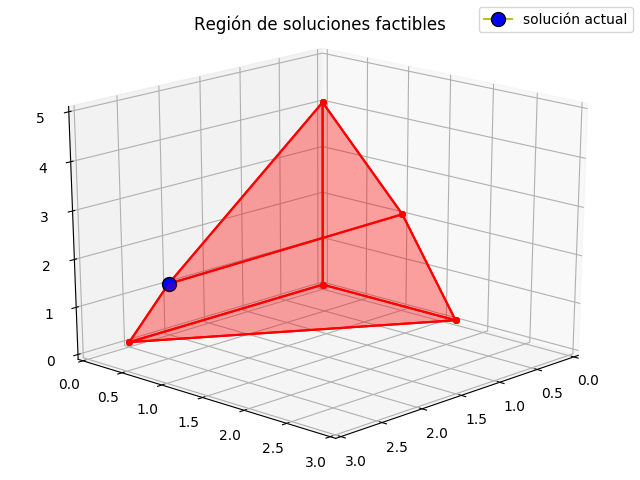
\includegraphics[scale=0.5]{imagenes/s3.png}
        \end{figure}
    \end{frame}

\end{document}


